\pagestyle{fancy}
\fancyhead{}
\fancyfoot{}
\renewcommand{\chaptermark}[1]{\markboth{\chaptername\ \thechapter\ \ \ \ {#1}}{}}
\renewcommand{\sectionmark}[1]{\markright{\thesection\ \ \ \  #1}}
\fancyhf{}         %Clears all header and footer fields, in preparation.
%\fancyheadoffset[LE,RO]{\marginparsep}
%\addtolength{\headwidth}{\marginparwidth}

%\ifthenelse{\boolean{sevenbytenbooksize}}{\fancyhfoffset[LE,RO]{30pt}}{}  
		%  CreateSpace text size but really not needed as its an ``else''
		%  from above
		
\fancyhfoffset[LE,RO]{30pt}
\fancyfoot[LE,RO]{\textbf{\thepage}} %Displays the page number in bold in the header,
                       % to the left on even pages and to the right on odd pages.
                                     
\fancyhead[LE]{\nouppercase{\leftmark}}
      %Displays the upper-level (chapter) information---
      % as determined above---in non-upper case in the header, 
      %to the right on even pages.
\fancyhead[RO]{\rightmark}
			%Displays the lower-level (section) information---as
      % determined above---in the header, to the left on odd pages.
\renewcommand{\headrulewidth}{0pt}
\renewcommand{\footrulewidth}{0pt}
	%Underlines the header and footer. (Set to 0pt if not required).

\makeatletter
\def\@makechapterhead#1{%
  {\parindent \z@ \raggedright \reset@font
    \large
    \resizebox{1.6cm}{2cm}{\thechapter}\ \ %
		\if \thechapter 1
%
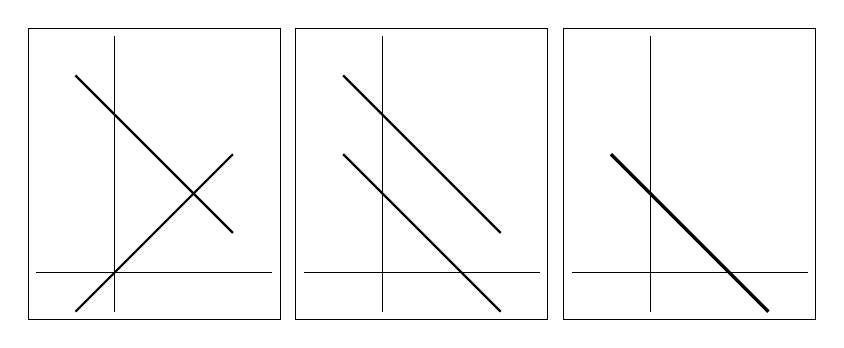
\begin{tikzpicture}
%Chapter 1 Pic 1
\begin{scope}
\draw (-1,0)--(2,0);
\draw (0,-.5)--(0,3);
\draw [thick] (-.5,-.5)--(1.5,1.5);
\draw [thick] (-.5,2.5)--(1.5,.5);
\draw  (-1.1,-.6)--(2.1,-.6)--(2.1,3.1)--(-1.1,3.1)--cycle;
\end{scope}

%Chapter 1 pic 2
\begin{scope}[shift={(3.4,0)}]
\draw (-1,0)--(2,0);
\draw (0,-.5)--(0,3);
\draw [thick] (-.5,1.5)--(1.5,-.5);
\draw [thick] (-.5,2.5)--(1.5,.5);
\draw  (-1.1,-.6)--(2.1,-.6)--(2.1,3.1)--(-1.1,3.1)--cycle;
\end{scope}

%Chapter 1 pic 3
\begin{scope}[shift={(6.8,0)}]
\draw (-1,0)--(2,0);
\draw (0,-.5)--(0,3);
\draw [very thick] (-.5,1.5)--(1.5,-.5);
%\draw [thick] (-.5,2.5)--(1.5,.5);
\draw (-1.1,-.6)--(2.1,-.6)--(2.1,3.1)--(-1.1,3.1)--cycle;
\end{scope}
\end{tikzpicture}
%
\else \if \thechapter 2
%
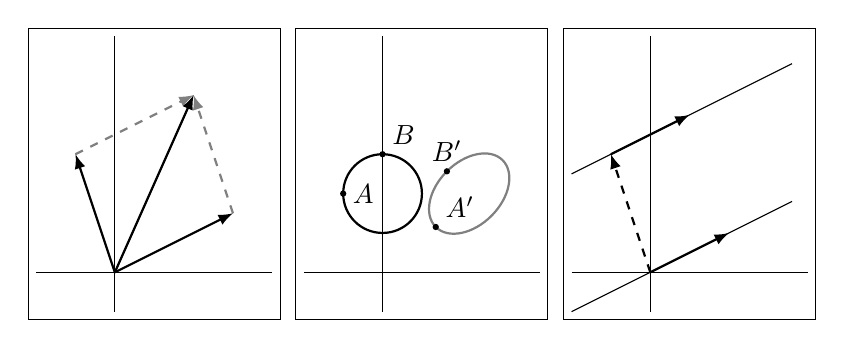
\begin{tikzpicture}[>=latex]

%chapter 2 pic 1
\begin{scope}
\draw (-1,0)--(2,0);
\draw (0,-.5)--(0,3);
\draw [thick,->] (0,0)--(-.5,1.5);
\draw [thick,->] (0,0)--(1.5,.75);
\draw [thick,->,dashed,gray] (-.5,1.5)--(1,2.25);
\draw [thick,->,dashed,gray] (1.5,.75)--(1,2.25);
\draw [thick,->] (0,0)--(1,2.25);
\draw  (-1.1,-.6)--(2.1,-.6)--(2.1,3.1)--(-1.1,3.1)--cycle;
\end{scope}

%Chapter 2 pic 2
\begin{scope}[shift={(3.4,0)}]
\draw (-1,0) -- (2,0);
\draw (0,-.5)--(0,3);
\draw [thick] (0,1) circle (.5cm);
\draw [thick, gray, rotate around={45:(1.1,1)}] (1.1,1) ellipse (.6cm and .4cm);
%\draw [thick,gray] (.6,1) node [right] {$A'$} .. (.6,.5) .. (1.65,1) .. (1.65,1.5) node [below left] {$B'$} ..cycle;
%\node [above] at (.817cm,1.28cm) {$A$};
%\fill (.817cm,1.28cm) circle (.04cm); 
\fill [rotate around={45:(1.1,1)}](.5,1) circle (.04cm) node [above right] {$A'$};
\fill [rotate around={45:(1.1,1)}](1.1,1.4) circle (.04cm) node [above ] {$B'$};

\fill (0,1.5) circle (.04) node [above right] {$B$}; 
\fill (-.5,1) circle (.04) node [right] {$A$};

\draw  (-1.1,-.6)--(2.1,-.6)--(2.1,3.1)--(-1.1,3.1)--cycle;
\end{scope}

%chapter 2 pic 3
\begin{scope}[shift={(6.8,0)}]
\draw (-1,0)--(2,0);
\draw (0,-.5)--(0,3);

\draw (-1,-.5)--(1.8,.9);
\draw [->,thick] (0,0)--(1,.5);
\draw [->,thick,dashed] (0,0)--(-.5,1.5);
\draw (-1,1.25)--(1.8,2.65);
\draw [->,thick] (-.5,1.5)--(.5,2);

\draw  (-1.1,-.6)--(2.1,-.6)--(2.1,3.1)--(-1.1,3.1)--cycle;\end{scope}
\end{tikzpicture}
%
\else \if \thechapter 3
%
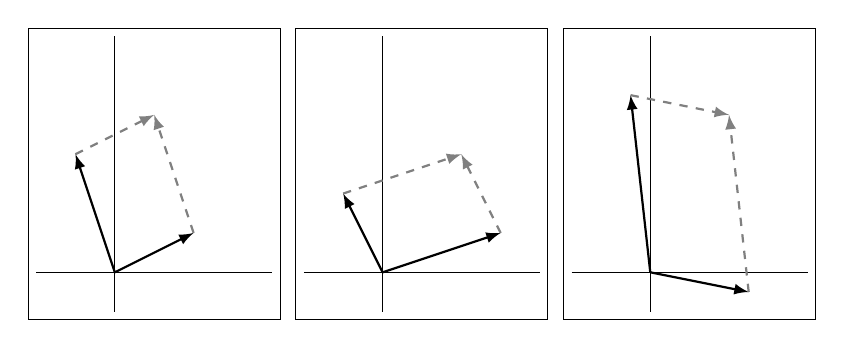
\begin{tikzpicture}[>=latex]

%chapter 3 pic 1
\begin{scope}
\draw (-1,0)--(2,0);
\draw (0,-.5)--(0,3);
\draw  (-1.1,-.6)--(2.1,-.6)--(2.1,3.1)--(-1.1,3.1)--cycle;

\draw [->,thick] (0,0)--(-.5,1.5);
\draw [->,thick] (0,0)--(1,.5);
\draw [->,thick,dashed,gray] (-.5,1.5)--(.5,2);
\draw [->,thick,dashed,gray] (1,.5)--(.5,2);

\end{scope}

%chapter 3 pic 2
\begin{scope}[shift={(3.4,0)}]
\draw (-1,0) -- (2,0);
\draw (0,-.5)--(0,3);
\draw  (-1.1,-.6)--(2.1,-.6)--(2.1,3.1)--(-1.1,3.1)--cycle;

\draw [->,thick] (0,0)--(-.5,1);
\draw [->,thick] (0,0)--(1.5,.5);
\draw [->,thick,dashed,gray] (-.5,1)--(1,1.5);
\draw [->,thick,dashed,gray] (1.5,.5)--(1,1.5);

\end{scope}

%chapter 3 pic 3
\begin{scope}[shift={(6.8,0)}]
\draw (-1,0)--(2,0);
\draw (0,-.5)--(0,3);
\draw  (-1.1,-.6)--(2.1,-.6)--(2.1,3.1)--(-1.1,3.1)--cycle;

\draw [->,thick] (0,0)--(1.25,-.25);
\draw [->,thick] (0,0)--(-.25,2.25);
\draw [->,thick,dashed,gray] (1.25,-.25)--(1,2);
\draw [->,thick,dashed,gray] (-.25,2.25)--(1,2);
\end{scope}

\end{tikzpicture}
%
\else \if \thechapter 4
%
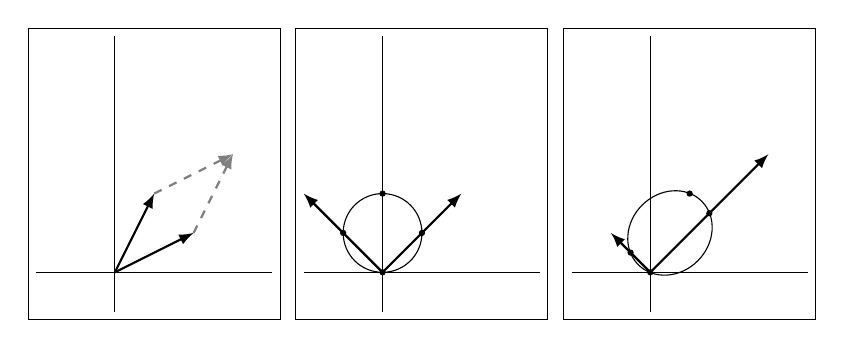
\begin{tikzpicture}[>=latex]

%chapter 4 pic 1
\begin{scope}
\draw (-1,0)--(2,0);
\draw (0,-.5)--(0,3);
\draw  (-1.1,-.6)--(2.1,-.6)--(2.1,3.1)--(-1.1,3.1)--cycle;

\draw [->,thick] (0,0)--(1,.5);
\draw [->,thick] (0,0)--(.5,1);
\draw [->,thick,dashed,gray] (1,.5)--(1.5,1.5);
\draw [->,thick,dashed,gray] (.5,1)--(1.5,1.5);

\end{scope}

%chapter 4 pic 2
\begin{scope}[shift={(3.4,0)}]
\draw (-1,0) -- (2,0);
\draw (0,-.5)--(0,3);
\draw  (-1.1,-.6)--(2.1,-.6)--(2.1,3.1)--(-1.1,3.1)--cycle;

\draw [->,thick] (0,0)--(-1,1);
\draw [->,thick] (0,0)--(1,1);
\draw (0,.5) circle (.5);
\fill (0,0) circle (.04); 
\fill (-.5,.5) circle (.04); 
\fill (.5,.5) circle (.04); 
\fill (0,1) circle (.04); 

\end{scope}

%chapter 4 pic 3
\begin{scope}[shift={(6.8,0)}]
\draw (-1,0)--(2,0);
\draw (0,-.5)--(0,3);
\draw  (-1.1,-.6)--(2.1,-.6)--(2.1,3.1)--(-1.1,3.1)--cycle;

\draw [->,thick] (0,0)--(-.5,.5);
\draw [->,thick] (0,0)--(1.5,1.5);
\fill (0,0) circle (.04); 
\fill (-.25,.25) circle (.04); 
\fill (.75,.75) circle (.04); 
\fill (.5,1) circle (.04); 
%\draw (.25,.5) circle (.55);

\draw [rotate around={45:(.25,.5)}] (.25,.5) ellipse (.57 and .5);

\end{scope}

\end{tikzpicture}
%
\else \if \thechapter 5
%
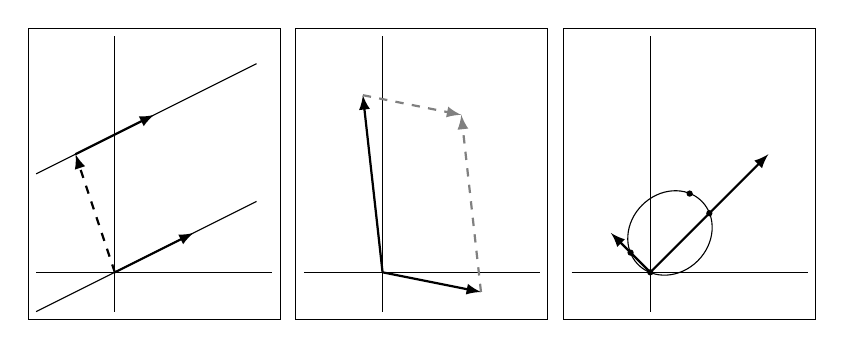
\begin{tikzpicture}[>=latex]

%chapter 5 pic 1
\begin{scope}
\draw (-1,0)--(2,0);
\draw (0,-.5)--(0,3);

\draw (-1,-.5)--(1.8,.9);
\draw [->,thick] (0,0)--(1,.5);
\draw [->,thick,dashed] (0,0)--(-.5,1.5);
\draw (-1,1.25)--(1.8,2.65);
\draw [->,thick] (-.5,1.5)--(.5,2);

\draw  (-1.1,-.6)--(2.1,-.6)--(2.1,3.1)--(-1.1,3.1)--cycle;
\end{scope}

%chapter 5 pic 2
\begin{scope}[shift={(3.4,0)}]
\draw (-1,0)--(2,0);
\draw (0,-.5)--(0,3);
\draw  (-1.1,-.6)--(2.1,-.6)--(2.1,3.1)--(-1.1,3.1)--cycle;

\draw [->,thick] (0,0)--(1.25,-.25);
\draw [->,thick] (0,0)--(-.25,2.25);
\draw [->,thick,dashed,gray] (1.25,-.25)--(1,2);
\draw [->,thick,dashed,gray] (-.25,2.25)--(1,2);
\end{scope}

%chapter 5 pic 3
\begin{scope}[shift={(6.8,0)}]
\draw (-1,0)--(2,0);
\draw (0,-.5)--(0,3);
\draw  (-1.1,-.6)--(2.1,-.6)--(2.1,3.1)--(-1.1,3.1)--cycle;

\draw [->,thick] (0,0)--(-.5,.5);
\draw [->,thick] (0,0)--(1.5,1.5);
\fill (0,0) circle (.04); 
\fill (-.25,.25) circle (.04); 
\fill (.75,.75) circle (.04); 
\fill (.5,1) circle (.04); 
%\draw (.25,.5) circle (.55);

\draw [rotate around={45:(.25,.5)}] (.25,.5) ellipse (.57 and .5);

\end{scope}

\end{tikzpicture}
%
\else \if \thechapter A
%
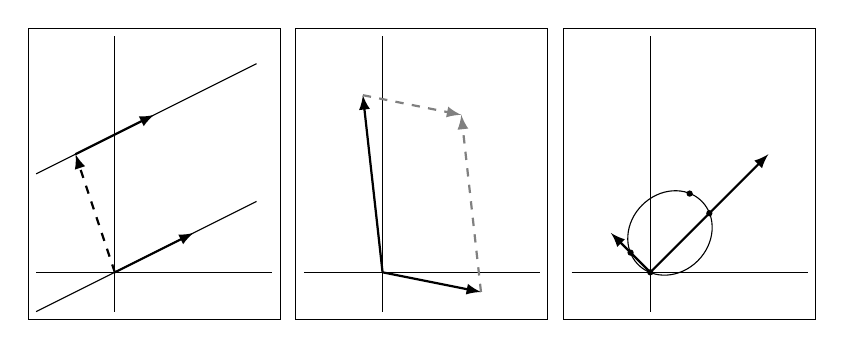
\begin{tikzpicture}[>=latex]

%appendix pic 1 = chapter 2 pic 3
\begin{scope}
\draw (-1,0)--(2,0);
\draw (0,-.5)--(0,3);

\draw (-1,-.5)--(1.8,.9);
\draw [->,thick] (0,0)--(1,.5);
\draw [->,thick,dashed] (0,0)--(-.5,1.5);
\draw (-1,1.25)--(1.8,2.65);
\draw [->,thick] (-.5,1.5)--(.5,2);

\draw  (-1.1,-.6)--(2.1,-.6)--(2.1,3.1)--(-1.1,3.1)--cycle;
\end{scope}

%appendix pic 2 = chapter 3 pic 3
\begin{scope}[shift={(3.4,0)}]
\draw (-1,0)--(2,0);
\draw (0,-.5)--(0,3);
\draw  (-1.1,-.6)--(2.1,-.6)--(2.1,3.1)--(-1.1,3.1)--cycle;

\draw [->,thick] (0,0)--(1.25,-.25);
\draw [->,thick] (0,0)--(-.25,2.25);
\draw [->,thick,dashed,gray] (1.25,-.25)--(1,2);
\draw [->,thick,dashed,gray] (-.25,2.25)--(1,2);
\end{scope}

%appendix pic 3 = chapter 4 pic 3
\begin{scope}[shift={(6.8,0)}]
\draw (-1,0)--(2,0);
\draw (0,-.5)--(0,3);
\draw  (-1.1,-.6)--(2.1,-.6)--(2.1,3.1)--(-1.1,3.1)--cycle;

\draw [->,thick] (0,0)--(-.5,.5);
\draw [->,thick] (0,0)--(1.5,1.5);
\fill (0,0) circle (.04); 
\fill (-.25,.25) circle (.04); 
\fill (.75,.75) circle (.04); 
\fill (.5,1) circle (.04); 
%\draw (.25,.5) circle (.55);

\draw [rotate around={45:(.25,.5)}] (.25,.5) ellipse (.57 and .5);

\end{scope}

\end{tikzpicture}

\fi
\fi
\fi
\fi
\fi
\fi


    \reset@font\LARGE\scshape\bfseries\strut \textsc #1
    \par\vskip 10\p@
    \hrule height 1pt
    \vskip 50\p@
  }}
  
%\makeatletter
\def\@makesectionhead#1{%
	 {\reset@font\LARGE\itshape\bfseries\strut #1 \thechapter.\thesection \ #1
	 }}
